%%%%%%%%%%%%%%%%%%%%%  kbb talk %%%%%%%%%%%%%%%%%%%%%%%%%%%%%%%
%%%%%%%%%%%%%%%%%%%%%%%%%%%%%%%%%%%%%%%%%%%%%%%%%%%%%%%%%%%%%%%

\documentclass[12pt,fleqn]{seminar}
\input{seminar.bug}
\pagestyle{empty}
\pdfhorigin=1truein
\pdfvorigin=1truein


% packages
\usepackage{ifpdf}
\usepackage{bm}
\usepackage{latexsym}
\usepackage{color}
\usepackage{pstricks}
\usepackage{ulem} %uwave
\usepackage{amsmath}

\usepackage{amssymb}
%\usepackage{float}
\usepackage{bm}
%\usepackage{wasysym}
%\usepackage[landscape]{geometry}
\usepackage{graphicx}
\usepackage{epstopdf}
\graphicspath{{./Figs/}{./}{../}}
\graphicspath{{/Users/danielhurowitz/PROJ/NEG/Figs/figs_for_paper/}{./}{../}}



% basic	commands I
\newcommand{\mass}{\mathsf{M}} 
\newcommand{\half}{\mbox{\small $\frac{1}{2}$}}
\newcommand{\sinc}{\mbox{sinc}}
\newcommand{\const}{\mbox{const}}
\newcommand{\trc}{\mbox{trace}}
\newcommand{\intt}{\int\!\!\!\!\int }
\newcommand{\ointt}{\int\!\!\!\!\int\!\!\!\!\!\circ\ }
\newcommand{\eexp}{\mbox{e}^}
\newcommand{\bra}{\left\langle}
\newcommand{\ket}{\right\rangle}
\newcommand{\EPS} {\mbox{\LARGE $\epsilon$}}
\newcommand{\ttimes} {\mbox{\tiny \ $^{\times}$ \ }}
\newcommand{\ar}{\mathsf r}
\newcommand{\im}{\mbox{Im}}
\newcommand{\re}{\mbox{Re}}
\newcommand{\bmsf}[1]{\bm{\mathsf{#1}}} 
\newcommand{\pd}[2]{\frac{\partial #1}{\partial #2}}
\newcommand{\bitem}{$\newline \ \ \bullet \ \ $} 
\newcommand{\ola}{\protect\overleftarrow}
\newcommand{\ora}{\protect\overrightarrow}

% basic	commands II
\newcommand{\hide}[1]{}
\newcommand{\tbox}[1]{\mbox{\tiny #1}}
\newcommand{\Cn}[1]{\begin{center}{#1}\end{center}}
\newcommand{\be}{\begin{eqnarray*}}
\newcommand{\ee}{\end{eqnarray*}}
\newcommand{\beq}{\begin{eqnarray*}}
\newcommand{\eeq}{\end{eqnarray*}}

\newcommand{\mpg}[2][0.45\hsize]{\begin{minipage}[b]{#1}{#2}\end{minipage}}
%
\newcommand{\bmp}[1]{\begin{minipage}[t]{#1}\noindent }
\newcommand{\smp}[1]{\end{minipage}\begin{minipage}[t]{#1}\noindent }
\newcommand{\emp}{\end{minipage}}

\newcommand{\amatrix}[1]{\begin{matrix} #1 \end{matrix}} 


% extra commands for colors
\definecolor{blk}{rgb}{0.,0.,0.}
\definecolor{red}{rgb}{1.,0.,0.}
\definecolor{green}{rgb}{0.,0.5,0.}
\definecolor{blue}{rgb}{0.,0.,1.}
\definecolor{bluek}{rgb}{0.,0.,0.5}
\definecolor{orange}{rgb}{1.,0.56.,0}
\newcommand{\cblk}[1]{\textcolor{blk}{#1}}
\newcommand{\cred}[1]{\textcolor{red}{#1}}
\newcommand{\cgreen}[1]{\textcolor{green}{#1}}
\newcommand{\cblue}[1]{\textcolor{blue}{#1}}
\newcommand{\cbluek}[1]{\textcolor{bluek}{#1}}
\newcommand{\corange}[1]{\textcolor{orange}{#1}}


% extra commands for slides

%\newcommand{\Up}[1][0.5]{\vspace{-#1cm}}
%\newcommand{\Dn}[1][0.5]{\vspace{#1cm}}
%\newcommand{\Tl}[1]{\begin{center}{\bf \small \cblue{#1}}\end{center}}

\newcommand{\Up}[1][5]{\vspace{-#1mm}}
\newcommand{\Dn}[1][5]{\vspace{#1mm}}
\newcommand{\Tl}[1]{\begin{center}{\bf \small \cblue{#1}}\end{center}}

\renewcommand{\slideparindent}{0mm}
\setlength{\mathindent}{0cm} 

% \newcommand{\newsld}{\end{slide}\begin{slide}}


\newcommand{\bslA}[1]{
%portrait
\pdfpagewidth=210truemm
\pdfpageheight=297truemm
\pdfhorigin=1truein
\pdfvorigin=1truein
%portrait
\renewcommand{\slidetopmargin}{0mm}
\renewcommand{\slideleftmargin}{-54mm}
\setlength{\slidewidth}{190mm}
\setlength{\slideheight}{277mm}
\begin{slide}
}



\newcommand{\bslB}[1]{
%landscape
\pdfpagewidth=297truemm
\pdfpageheight=210truemm
\pdfhorigin=1truein
\pdfvorigin=1truein
%portrait 
\renewcommand{\slidetopmargin}{0mm}
\renewcommand{\slideleftmargin}{33mm}
\setlength{\slideheight}{190mm}
\setlength{\slidewidth}{150mm} %130
%portrait fonts
\begin{slide}
\ptsize{8}
}



\newcommand{\bslC}[1]{
%landscape
\pdfpagewidth=297truemm
\pdfpageheight=210truemm
\pdfhorigin=1truein
\pdfvorigin=1truein
%landscape
\renewcommand{\slidetopmargin}{0mm}
\renewcommand{\slideleftmargin}{33mm}
\setlength{\slideheight}{190mm}
\setlength{\slidewidth}{277mm}
%portrait fonts
\begin{slide}
\ptsize{8}
}



\newcommand{\bslD}[1]{
%landscape
\pdfpagewidth=297truemm
\pdfpageheight=210truemm
\pdfhorigin=1truein
\pdfvorigin=1truein
%landscape
\renewcommand{\slidetopmargin}{0mm}
\renewcommand{\slideleftmargin}{33mm}
\setlength{\slideheight}{190mm}
\setlength{\slidewidth}{277mm}
%landscape fonts
\begin{slide}
}



\newcommand{\esl}{\end{slide}}


\newcommand{\vbar}{
\begin{picture}(1,1)
\thicklines
\put(0,61){ \ \ \line(0,-1){280} \ \ } 
\end{picture} 
}


%%%%%%%%%%%%%%%%%%%%%%%%%%%%%%%%%%%%%%%%%%%%%%%%%%%%%%%%%%%%%%%%%%%
%%%%%%%%%%%%%%%%%%%%%%%%%%%%%%%%%%%%%%%%%%%%%%%%%%%%%%%%%%%%%%%%%%%


%%%%%%%%%%%%%%%%%%%%%%%%%%%%%%%%%%%%%%%%%%%%%%%%%%%%%%%%%%%%%%%%%%%
%%%%%%%%%%%%%%%%%%%%%%%%%%%%%%%%%%%%%%%%%%%%%%%%%%%%%%%%%%%%%%%%%%%
\begin{document}
%%%%%%%%%%%%%%%%%%%%%%%%%%%%%%%%
\bslD

\Tl{\Large{Percolation, sliding, localization and relaxation in glassy circuits }}


\Cn{\bf Daniel Hurowitz, Doron Cohen\\ \corange{Ben-Gurion University}}
%
%
%\bmp{0.5\hsize}
%
%
%
%%\Cn{ \includegraphics[ height=4cm]{}}
%
%\smp{0.5\hsize}
%
%\vspace{0.2cm}
%
%
%
%%{\includegraphics[height=3cm]{ResistorsNetworkBath_a}}
%
%\emp
%
%\bmp{\hsize}



\bmp{0.5\hsize}

\Cn{
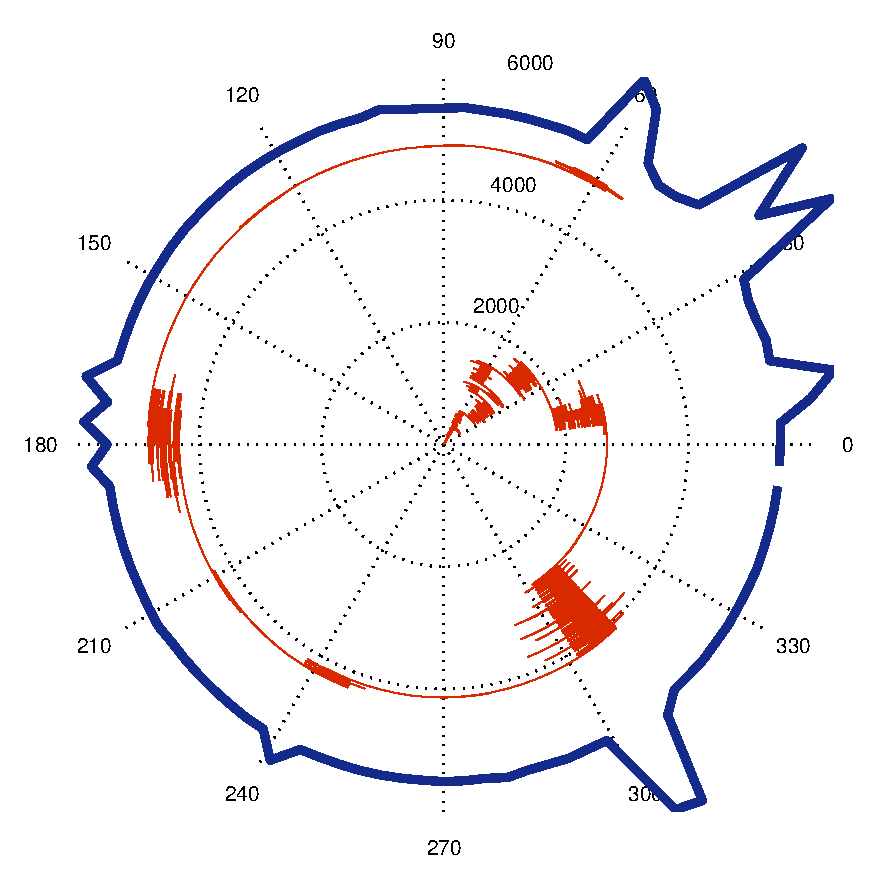
\includegraphics[height=4cm]{/Figs/polar_1_a.eps}

``Localized"
}

\smp{0.5\hsize}

\Cn{
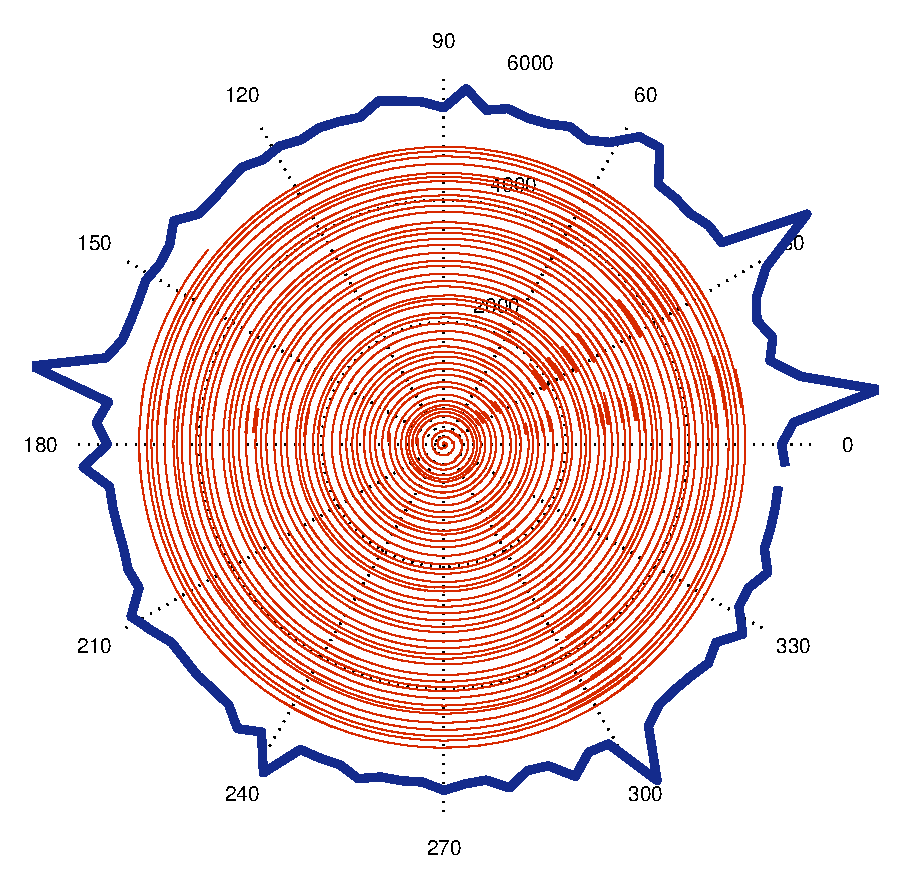
\includegraphics[height=4cm]{/Figs/polar_2_a.eps}

Sliding}

\emp

%\center{{   D. Hurowitz and D. Cohen, \texttt{arXiv} (2014)}}


%\emp

\esl


%%%%%%%%%%%%%%%%%%%%%%%%%%%%%%%%
\bslC

\Tl{\large Brownian motion}


\bmp{0.6\hsize}


\cgreen{{\bf Simple random walk} [Einstein]} 

\vspace{0.1cm}

Uniform lattice - all rates are equal $w$,

$\displaystyle D = a^2 w$

\smp{0.4\hsize}

\vspace{0.2cm}

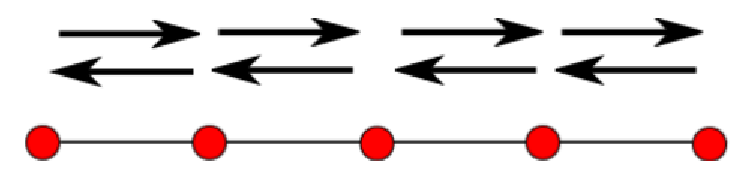
\includegraphics[width=4.5cm]{rw1a}

\emp

\vspace{0.1cm}


\bmp{0.6\hsize}

\cgreen{{\bf Random walk on disordered lattice} [Alexander et al.]} 

\vspace{0.1cm}

Random lattice - random, symmetric transition rates $w_n$

$P(w) \propto w^{\alpha-1}$ (for small $w$)

 $D = \text{resistor network calculation}$

{\bf Percolation} related transition to subdiffusion for 

$D=0$ for $\alpha<1$

\smp{0.4\hsize}

\emp

\vspace{0.1cm}

\bmp{0.61\hsize}

\cgreen{{\bf Random walk in random environment} [Sinai, Derrida, ...]} 

\vspace{0.1cm}

Rates allowed to be asymmetric $\displaystyle {\ora{w}_n}/{\ola{w}_n} = e^{\mathcal{E}_n}$

Stochastic field: $\mathcal{E}_n \sim [s-\sigma, \ s+\sigma]$

{\bf Sliding} transitions for $\displaystyle \left\langle e^{-\mathcal{E} \mu} \right\rangle =1$  (defines $s_{\mu}$)

$D=0$ for $s<s_{1/2}$

 $v=0$ for $s<s_1$


\smp{0.4\hsize}

\vspace{1cm}

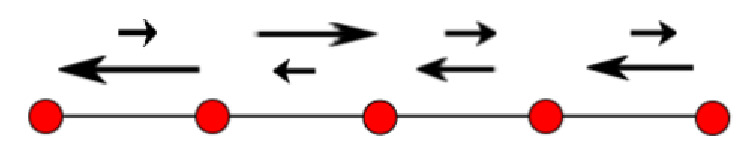
\includegraphics[width=4.5cm]{rw2a}

\emp

\Dn

\Cn{\large{\cred{\bf Implications of the percolation and sliding transitions on relaxation modes of closed ring}}}

\esl

\bslC

\Tl{\large Dynamics}

\bmp{0.6\hsize}

\cgreen{\bf Conservative rate equation}
%

\vspace{0.2cm}

\Cn{
$\displaystyle
\frac{d\bm{p}}{dt} \ \ = \ \ \bm{W} \bm{p},  \ \ \ \ \ 
\bm{W} \ \ = \ \ \left[\amatrix{
-\gamma_1   & w_{1,2}   & 0         & ... \\ 
w_{2,1}     & -\gamma_2 & w_{2,3}   & ... \\ 
0           & w_{3,2}   & -\gamma_3 & ... \\
...         & ...       & ...       & ...
}\right],
$
}

\vspace{.7cm}

\text{Transition rates across $n^{th}$ bond $w_n\eexp{\pm\mathcal{E}_n/2}$}

\vspace{0.1cm}

\text{Stochastic field $\mathcal{E}_n \sim [s-\sigma, \ s+\sigma] $}

\vspace{0.1cm}

\text{Resistor network $ P(w) \propto w^{\alpha-1}$}

\vspace{0.1cm}

\text{Affinity (closed ring) $ S_{\circlearrowleft} \ \ = \ \ \sum_{n=1}^N \mathcal{E}_n\ \ = \ \  Ns$}


\smp{0.4\hsize}


\Dn

%
\beq
&&\sum_{n=1}^N w_{nm} = 0\\
&&\text{i.e.}  \ \gamma_2 = w_{1,2}+w_{3,2}
\eeq

\Dn

\Cn{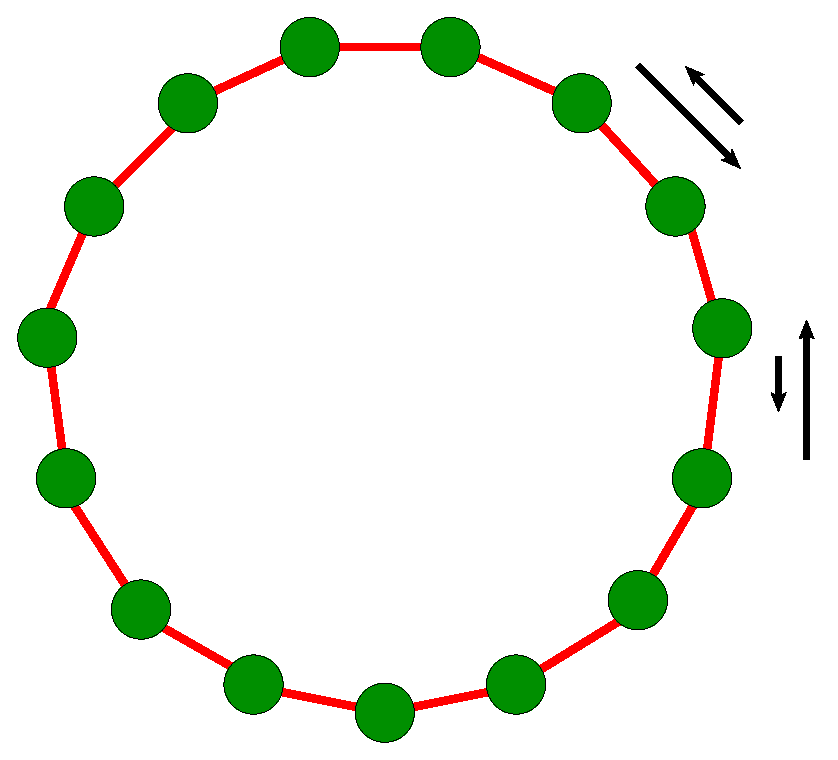
\includegraphics[height=3.cm]{sparse_network2.eps}}

\emp



\cgreen{\bf How do spectral properties of ${\bm W}$ depend on {$(\alpha,\sigma, s)$?}}

\begin{itemize}

\item \cred{\bf What is the threshold bias $s_c$ for complex eigenvalues (delocalization)?}

\item \cred{\bf How is $s_c$ related to the percolation transition? to the sliding transition?}

\item \cred{\bf Implications of conservativity?}

\end{itemize}


\esl


%%%%%%%%%%%%%%%%%%%%%%%%%%%%%%%%%%%%%%%%%%
\bslC

\Tl{\large The spectrum}

\bmp{0.33\hsize}

{
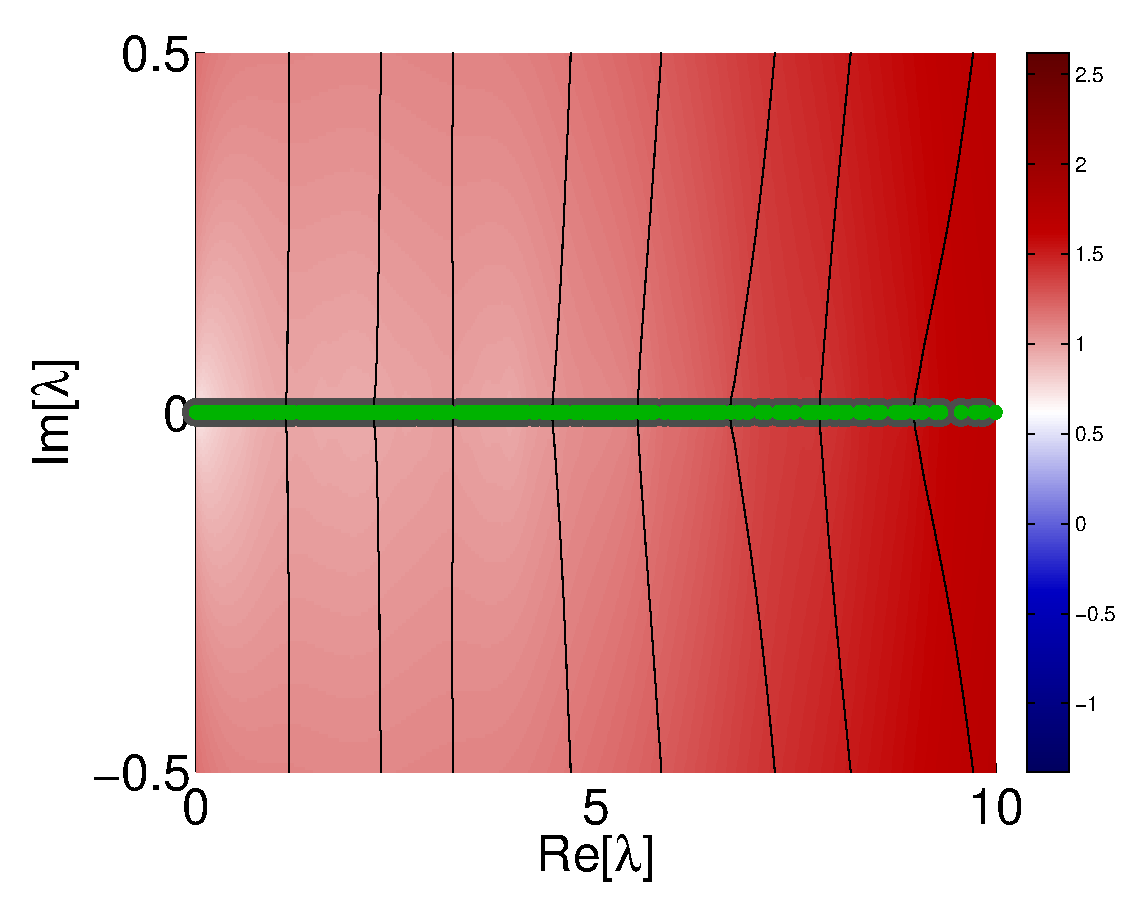
\includegraphics[height=3.5cm]{spectrum_electrostatics1_2}
}

\smp{0.33\hsize}

{
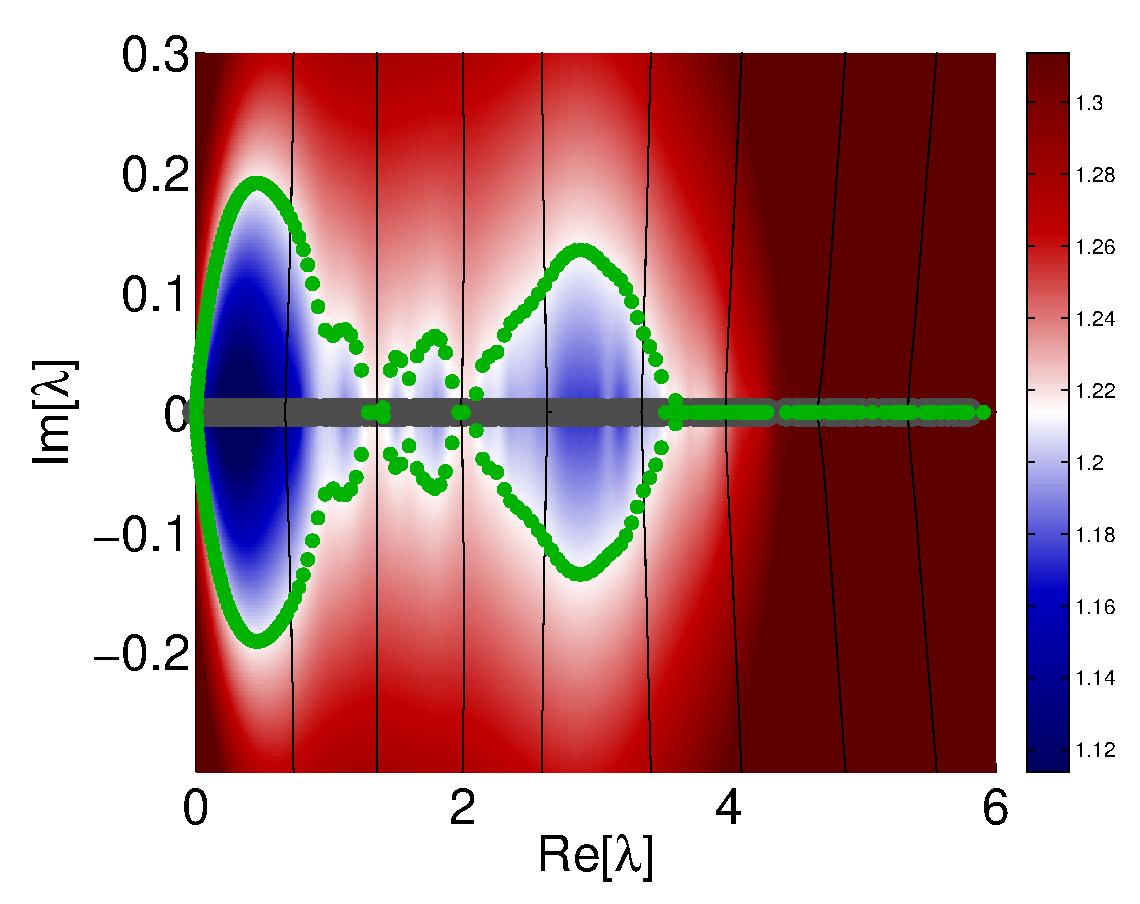
\includegraphics[height=3.5cm]{spectrum_electrostatics1}
}

\smp{0.33\hsize}

{
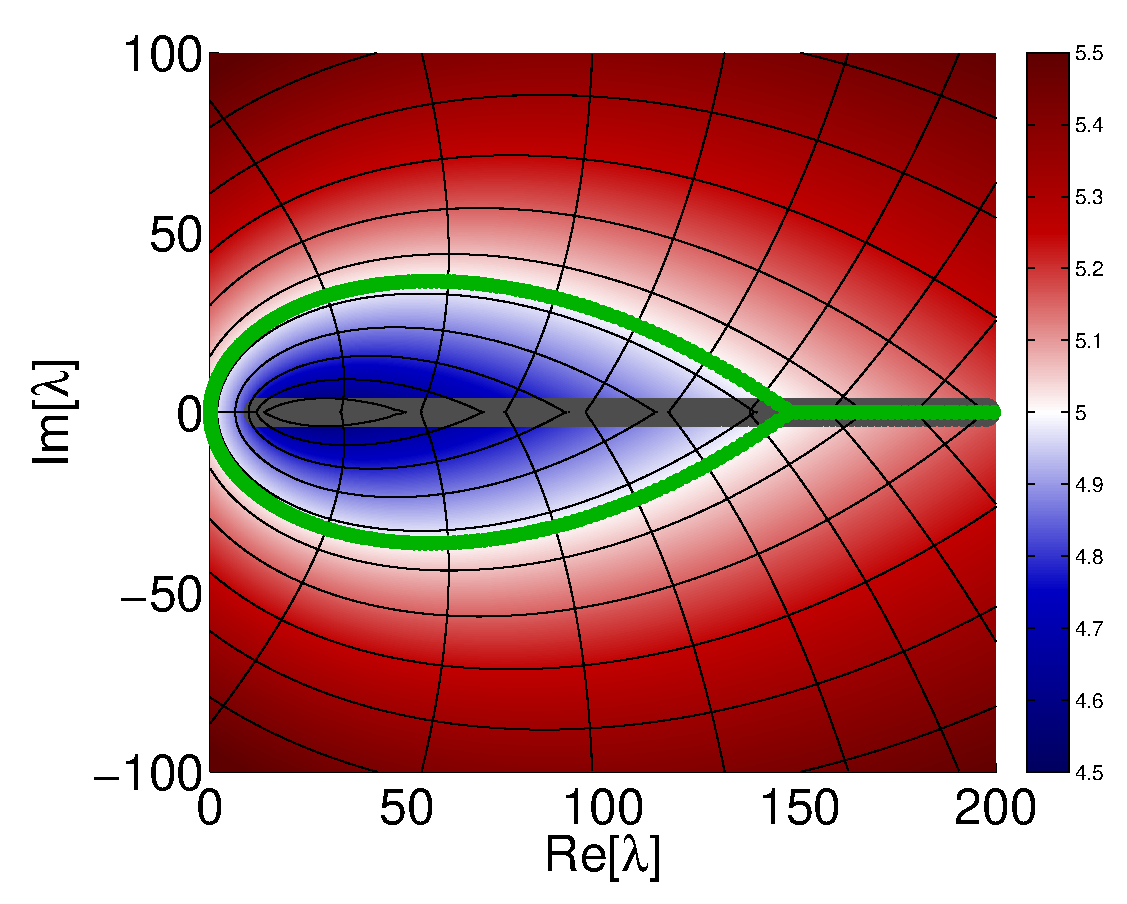
\includegraphics[height=3.5cm]{spectrum_electrostatics2}
}

\emp


\bmp{0.5\hsize}

\cgreen{\bf Observations}

\begin{itemize}

\item $\lambda_0 = 0$ due to conservativity

\item Complex eigenvalues $\leadsto$ oscillating density

\item Complex bubble at bottom of band

\item Complexity saturation

\end{itemize}

\smp{0.5\hsize}

\hspace{0.5cm}
%
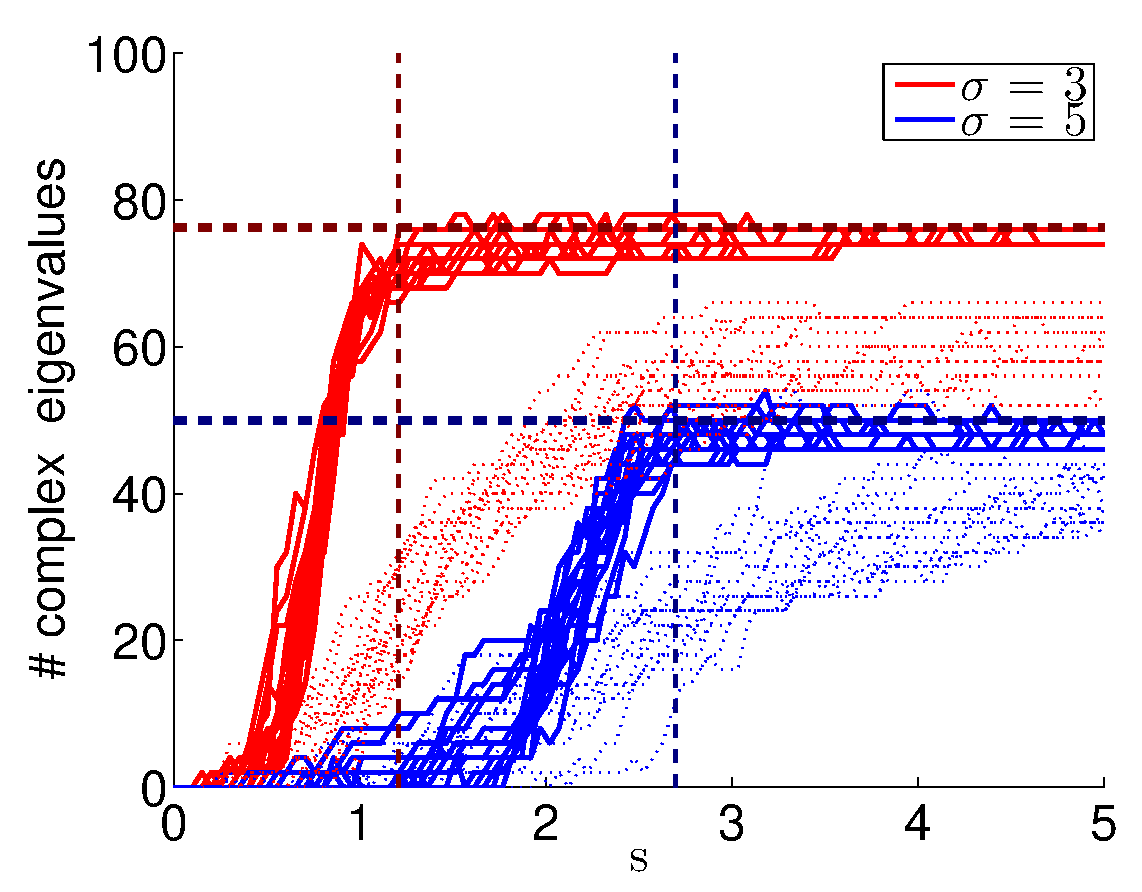
\includegraphics[height=3.5cm]{numComplex_100_alpha_sigma}


\emp

%\Cn{
%
%\cred{\bf What is the threshold bias $s_c$ for complex eigenvalues (delocalization)?}
%
%\cred{\bf How is $s_c$ related to the percolation transition? to the sliding transition?}
%}


\esl
%%%%%%%%%%%%%%%%%%%%%%%%%%%%%%%%%%%%%%%%%%%%%%%%%



%%%%%%%%%%%%%%%%%%%%%%%%%%%%%%%%%%%%%%%%%%

\bslC

\Tl{\large The spectral equation}


{
\cgreen{\bf Equation for eigenvalues }
% 
\Cn{
$\displaystyle 
\det (z-\bm{W})  =  \prod_{k=0}^{N-1} \left(z-\lambda_k\right) \ \ = \ \ 0
$
}


\cgreen{\bf Gauge away disorder} (imaginary AB flux)

{
$
{{\bm{\tilde{W}}} = \eexp{{\bm{U}/2}} \bm{W} \eexp{-{\bm{U}/2}}}
$

$\displaystyle
\tilde{\bm{W}} \ = \ 
\text{diagonal}\Big\{-\gamma_{n}\Big\} 
+\text{offdiagonal}\Big\{  w_{n}\eexp{\pm \frac{S_{\circlearrowleft}}{2N}}  \Big\}
$

\begin{itemize}

\item  \cred{\bf Cannot gauge away asymmetry $\mathcal{S}_{\circlearrowleft}$} (cannot gauge away flux in closed loop)

\item Off diagonal elements depend on $(\alpha,S_{\circlearrowleft})$

\item Diagonal elements depend on $(\alpha, \sigma, s)$  (conservativity)

\end{itemize}


}

\cgreen{\bf Associated Hermitian matrix ${\bm H}$ }

Set  ${S}_{\circlearrowleft} =0$ for off diagonal elements

${\bm H}$ is symmetric with real eigenvalues $\epsilon_k(s)$

\Cn{
{\bf Express spectral equation in terms of $\epsilon_k$} [1]

$\displaystyle
\prod_{k=0}^{N-1} \left(\frac{z+\epsilon_k(s)}{\overline{w}}\right) \ \ = \ \ 2\left[\cosh\left(\frac{S_{\circlearrowleft}}{2}\right)-1\right]
$


}
}
%
%
\Dn

\footnotesize{[1] N.M. Shnerb, D.R. Nelson, Phys. Rev. Lett. 80, 5172 (1998)}

\esl

%%%%%%%%%%%%%%%%%%%%%%%%%%%%%%%%%%
\bslC

\Tl{\large Spectrum of ${\bm H}$}

\vspace{0.2cm}


{${\bm H}$ is a symmetric matrix with real eigenvalues $\epsilon_k (s) \in [\epsilon_s, \ \epsilon_{\infty}]$}

\vspace{0.2cm}

\cgreen{\bf Clean ring} - gapped spectrum $\displaystyle \epsilon_{s,\infty} = 2 \left[ \cosh(s/2) \mp 1 \right]$


\cgreen{\bf Sparse disorder} ($M \ll N$ defects) - Few eigenvalues isolated from the continuum

\Dn

\cred{{\bf Fully disordered ring}} - 
Gap closes, 
%
densifty of states 
$
\ \ \rho(\epsilon) \ \propto \ \epsilon^{\cred{\mu}-1} \ \ \ \ \text{(for small $\epsilon$)}
$

\vspace{-0.3cm}

\bmp{0.5\hsize}

\cgreen{\bf Stochastic field disorder}

\vspace{0.2cm}

{\bf Gaussian disorder} [1] \ \  $\displaystyle {s=\frac{1}{2} \sigma^2 \cred{\mu}}$ 


{\bf Box disorder }
%
$\displaystyle
s \ = \ s_{\cred{\mu}} \ = \ \frac{1}{\cred{\mu}} \ln\left( \frac{\sinh (\sigma\cred{\mu})}{\sigma\cred{\mu}} \right)
$

\vspace{0.1cm}

For $s>s_{\infty} = \sigma$, gap opens, $\epsilon_s = \eexp{(s-\sigma)/2}$




\Dn

\cgreen{\bf Resistor network disorder} [2]

\vspace{0.2cm}

$\displaystyle
 \cred{\mu} = \text{min} \left\{ \frac{\alpha}{1+\alpha}, \ \frac{1}{2} \right\}
 $

\vspace{.2cm}

For large bias,  ${\bm H}$ is trivially localized, $\cred{\mu}=\alpha$


\smp{0.5\hsize}

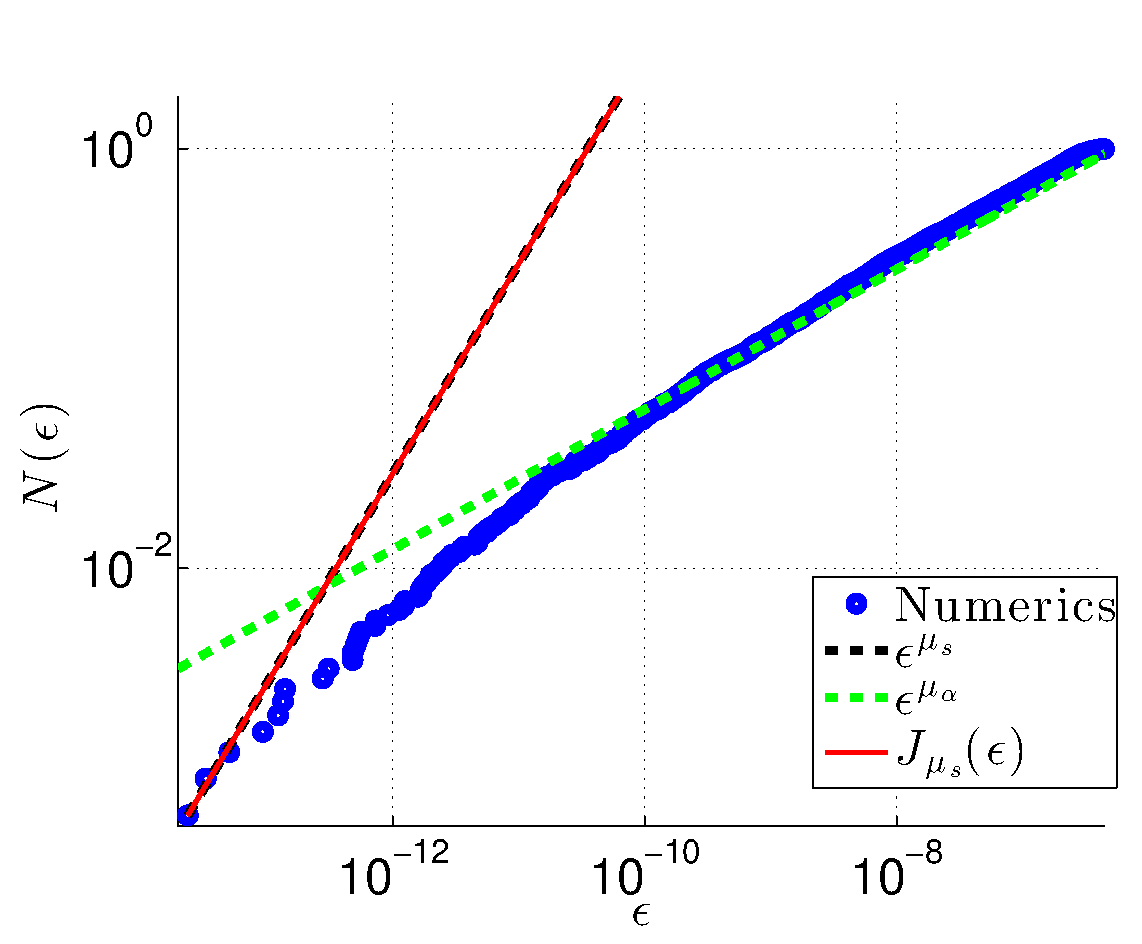
\includegraphics[height=3.5cm]{N_E_1_1_french}

Resistor network modifies spectral density at high energies

\emp

\Dn

\footnotesize{
[1] J. Bouchaud, A. Comtet, A. Georges, and P. L. Doussal, Annals
of Physics 201, 285 (1990)

[2]  S. Alexander, J. Bernasconi, W. R. Schneider, and R. Orbach,
Rev. Mod. Phys. 53, 175 (1981).}



\esl

%%%%%%%%%%%%%%%%%%%%%%%%%%%%%%%%%%%%%%%%%%

\bslC

 

\Tl{\large Electrostatic picture}

\vspace{0.1cm}
%set $\overline{w}=1, \  z \mapsto -z$

2D Electrostatic potential
%
$\displaystyle \ 
\Psi(z) \ \ = \ \ \sum_k \ln\left(z-\epsilon_k\right) \ \ \equiv \ \ V(x,y)+iA(x,y)
$

The secular equation
%
$\displaystyle
\ \ \ \ \ \ V(x,y)=V(0) \ \ \ \ A(x,y)=2\pi*\text{integer} 
$

\vspace{0.1cm}

\Cn{
\cred{\bf Condition for complexity $V(\epsilon) < V(0)=\ln\left[ 2(\cosh(S_{\circlearrowleft}/2)-1)\right];$}
}


\cgreen{\bf Continuum approximation}

Density of states $\iff$ charge density $\rho \propto \epsilon^{\mu-1}$ along real axis

Potential along real axis
%
$\displaystyle
V(\epsilon) \ \ = \ \  \int \ln \left(|\epsilon-x' \right|) \rho(x')dx' \ \ \ \ \text{}
$

Derivative at origin
%
$\displaystyle
 \ \ \ \ \ \  V'(\epsilon) \ \ \approx  \ \ \frac{ \epsilon^{\mu-1}}{\epsilon_c^{\mu}} \pi \mu \cot(\pi \mu)
$
, {\bf changes sign at $\mu=1/2$}


\vspace{0.1cm}

\Cn{
\cred{\bf Condition for complexity $V'(\epsilon) < 0$}
}


\bmp{0.33\hsize}

{
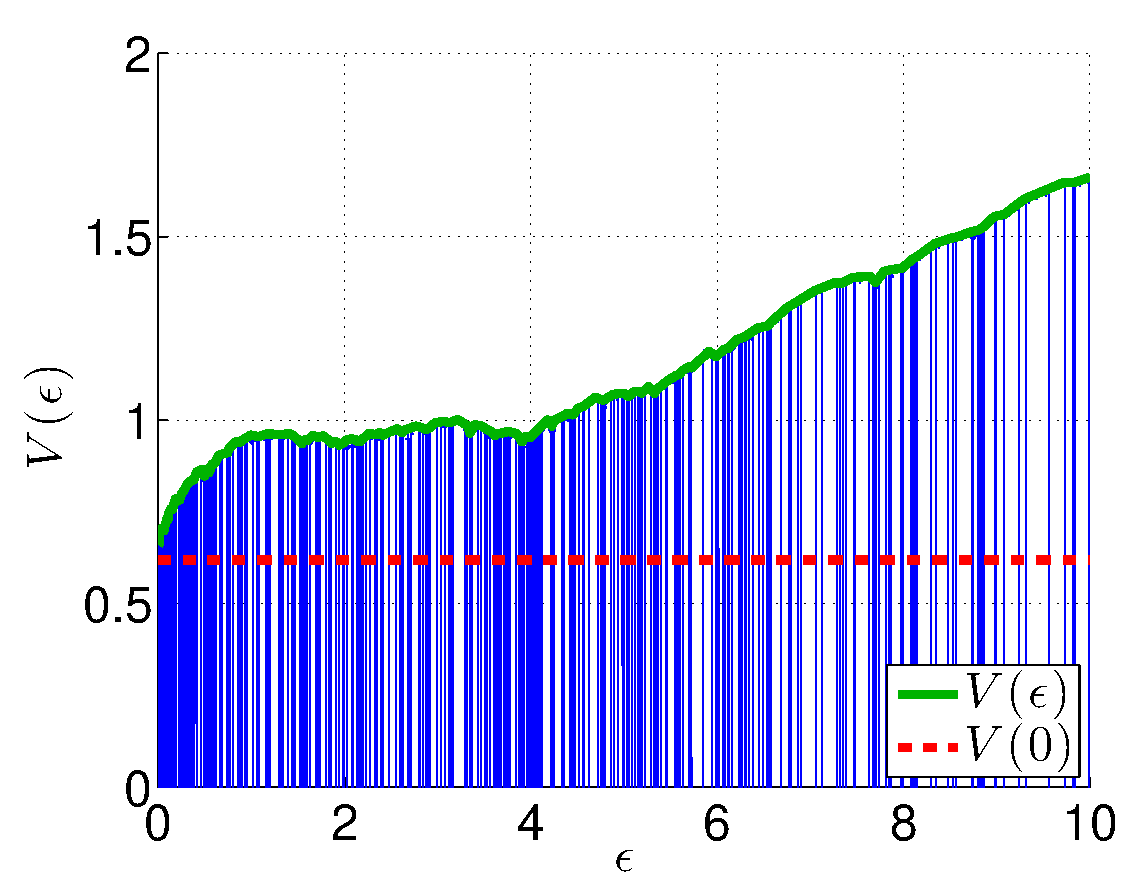
\includegraphics[height=3cm]{V_E_1_2b}

\Cn{$s<s_{1/2}$}

}

\smp{0.33\hsize}

{
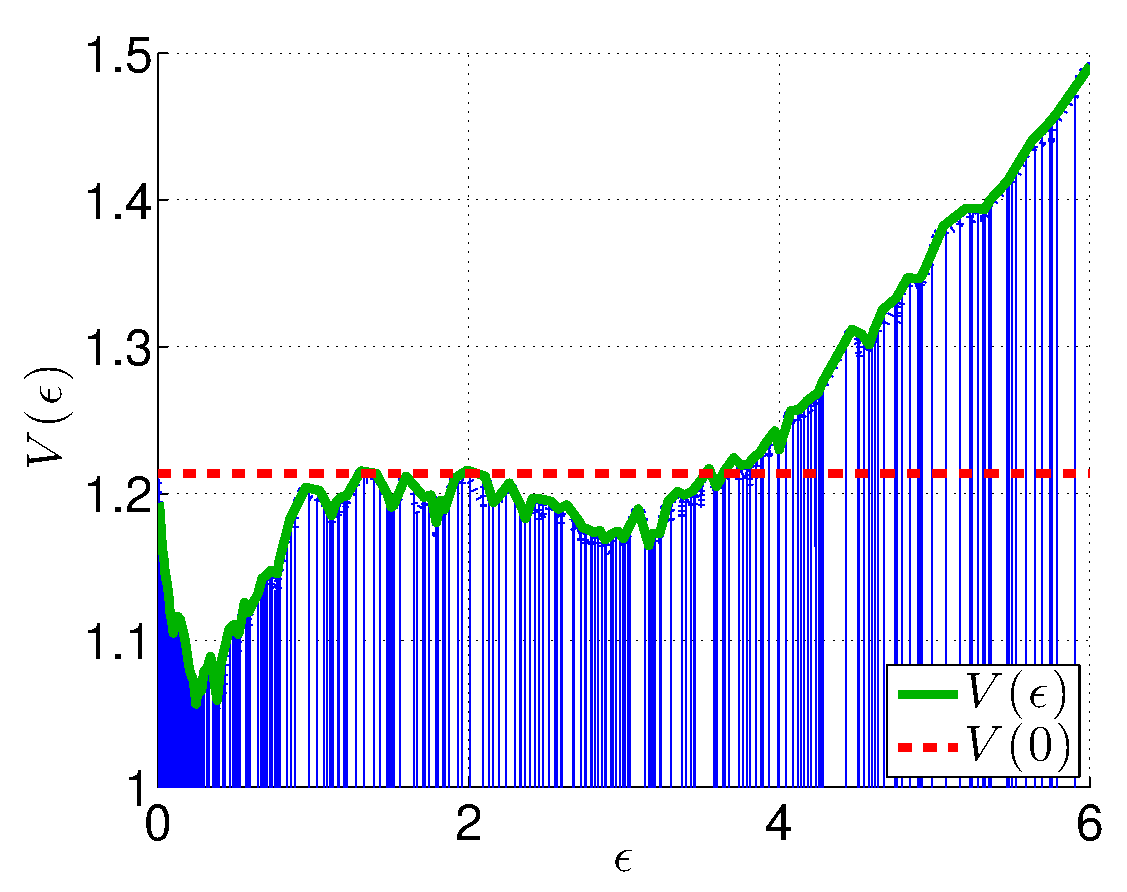
\includegraphics[height=3cm]{V_E_1b}

\Cn{$s>s_{1/2}$}

}

\smp{0.33\hsize}

{
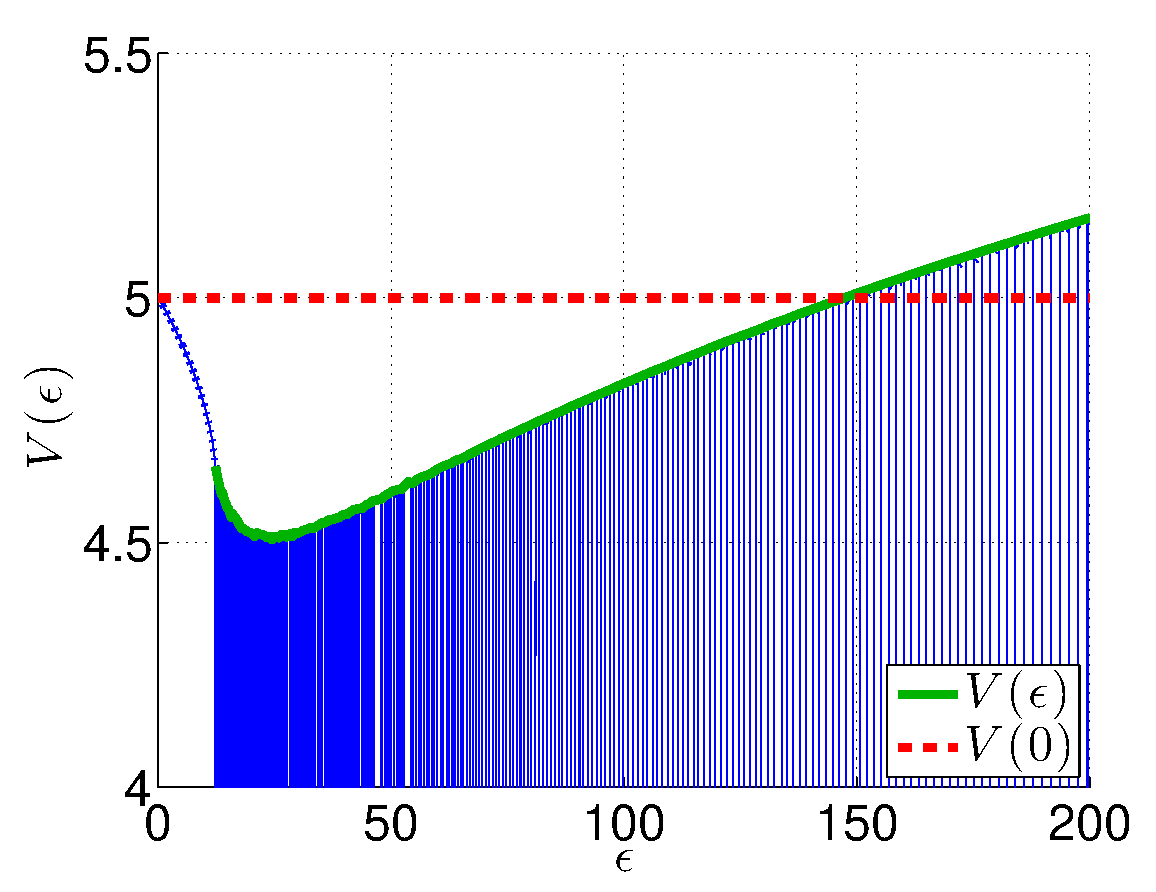
\includegraphics[height=3cm]{V_E_2b}

\Cn{$s>s_{\infty}$}

}



\emp

\esl

\bslC

\Tl{\large Complexity threshold bias}

\bmp{0.6\hsize}

\cgreen{\bf Stochastic field, $\mu=\mu_s(\sigma)$}

\vspace{0.2cm}

$\displaystyle s_c = s_{1/2} < s_1$

\Dn



\cgreen{\bf Resistor network, $\mu=\mu_{\alpha}$}



\beq
\left\{ 
\begin{matrix}
s=0 & \text{resistor network} & \Longrightarrow & \ \ \ \ \mu \ = \ \frac{\alpha}{1+\alpha} \\
\text{large}  \  s & \text{trivial localization} & \Longrightarrow & \mu \ = \ \alpha
\end{matrix}
\right.
\eeq

\beq
\alpha &<& 1/2 \Rightarrow s_c = \infty\\
\alpha &>& 1/2 \Rightarrow s_c \sim 1/N\ \ \ \text{[Numerically verified]}
\eeq

\Dn

\cgreen{\bf Sparse disorder}

\vspace{0.2cm}

Clean ring with  $M \ll N$ defects

\vspace{0.1cm}

$s_c \sim 1/N \ll s_1$

\vspace{0.1cm}

For $M$ field defects $s_c= \sigma \sqrt{M}/N$

\smp{0.4\hsize}

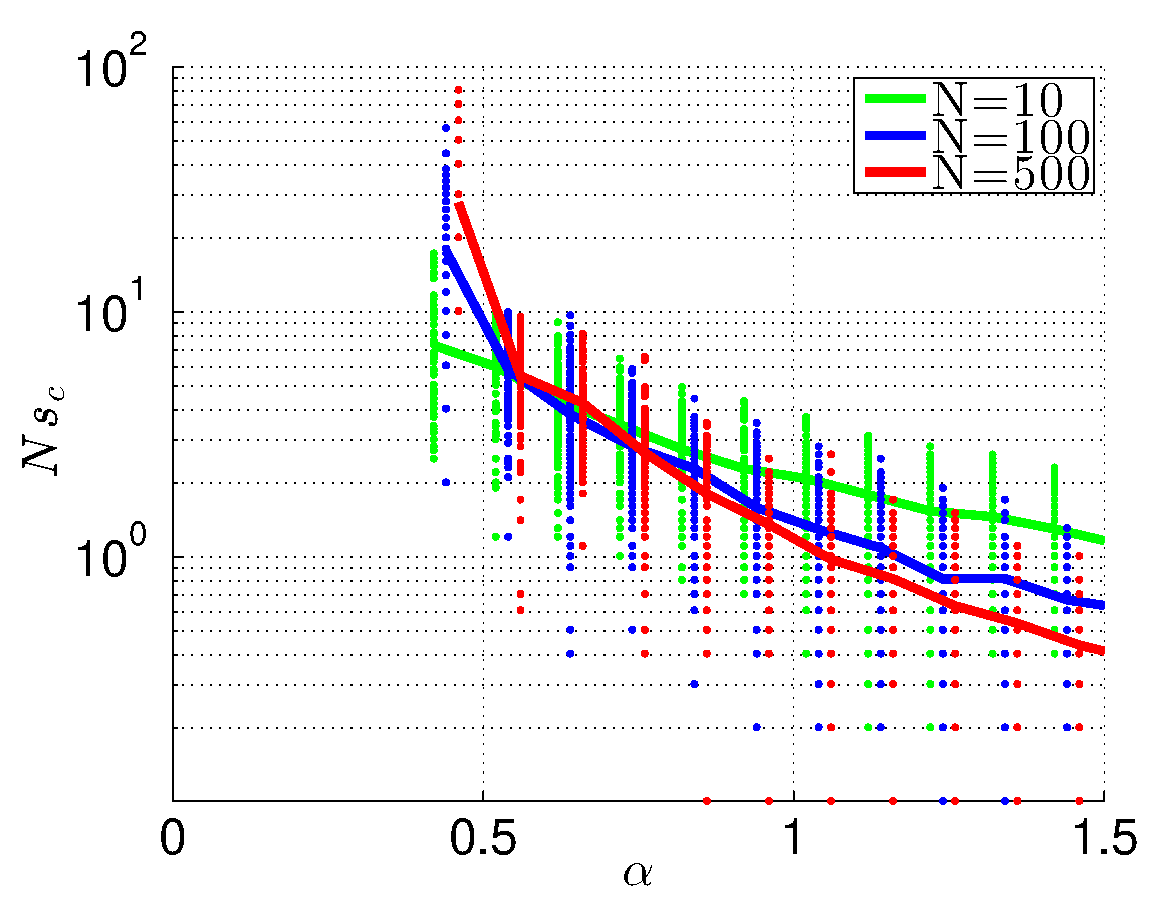
\includegraphics[height=4cm]{s_c_vs_alpha}


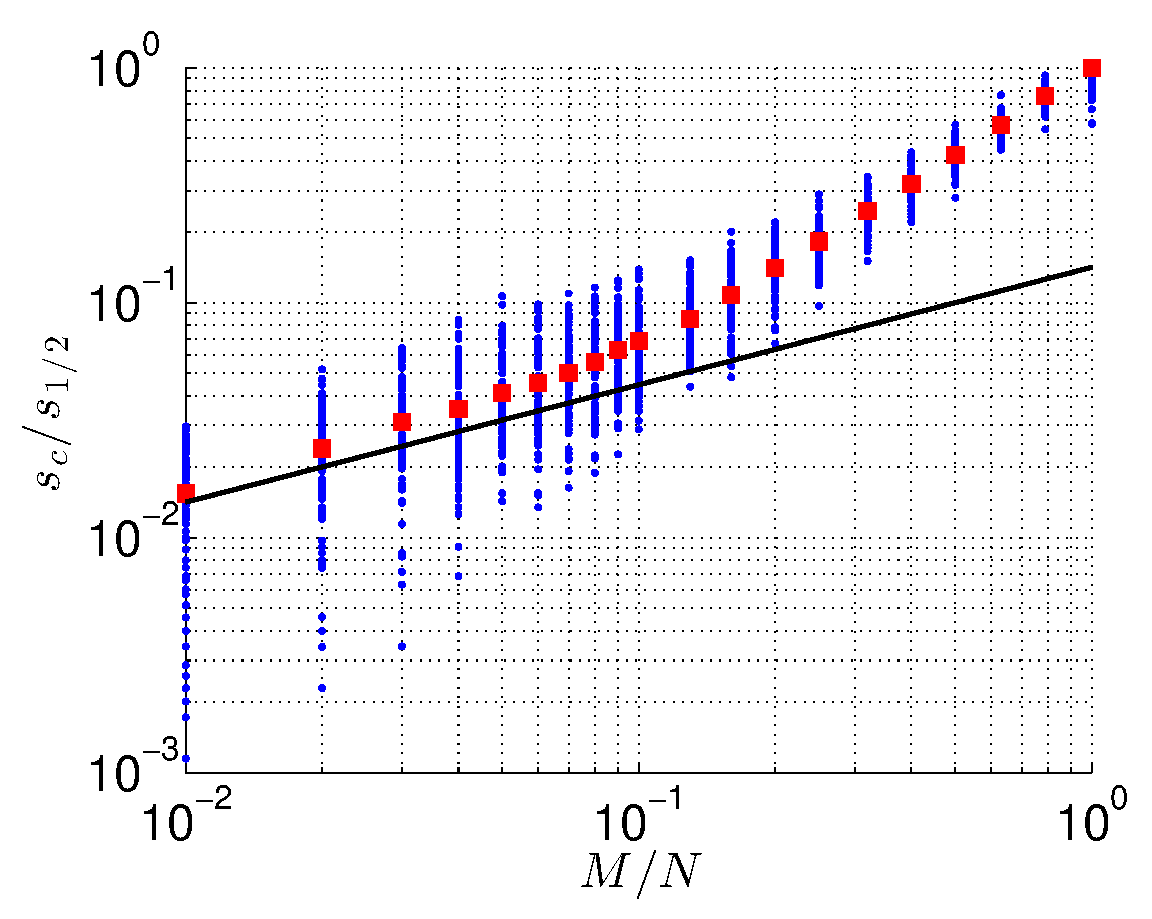
\includegraphics[height=4cm]{s_c_sparse_100_loglog}

\emp


\esl

\bslC

\Tl{\large Complexity saturation}

\cgreen{\bf Recall the spectral determinant}
%
\Cn{
$\displaystyle
\ \ \prod_{k=0}^{N-1} \left(\frac{z+\epsilon_k(s)}{\overline{w}}\right) \ \ = \ \ 2\left[\cosh\left(\frac{S_{\circlearrowleft}}{2}\right)-1\right], \ \ \ \ 
S_{\circlearrowleft} = sN$
}

\bmp{0.6\hsize}

\cgreen{\bf For large $s$ }


{\bf Non conservative}

LHS, RHS are independent   
%
$\leadsto$  \text{entirely complex spectrum}

\Dn

{\bf Conservative} 

$ \epsilon_n \ = \ \gamma_n \ = \ w_n \eexp{\mathcal{E}_n/2} \sim \eexp{s}$

$\text{LHS, RHS }\sim \eexp{sN/2}$
%
$\leadsto$  \text{complexity saturation}

%

\Dn

\cgreen{\bf The saturation fraction}

{Upper cutoff $\epsilon_c$ determined by} $\overline{\ln\left[ \epsilon - w\eexp{\mathcal{E}/2} \right]} \ \ = \ \ s/2$

{Count number of eigenvalues up to}  $\epsilon_c$

\Dn

{\bf Gaussian disorder}

 $V(\epsilon\to\infty) = \const $  

Enitrely complex spectrum 

Sharp transition at $s=s_{1/2}$





\smp{0.4\hsize}



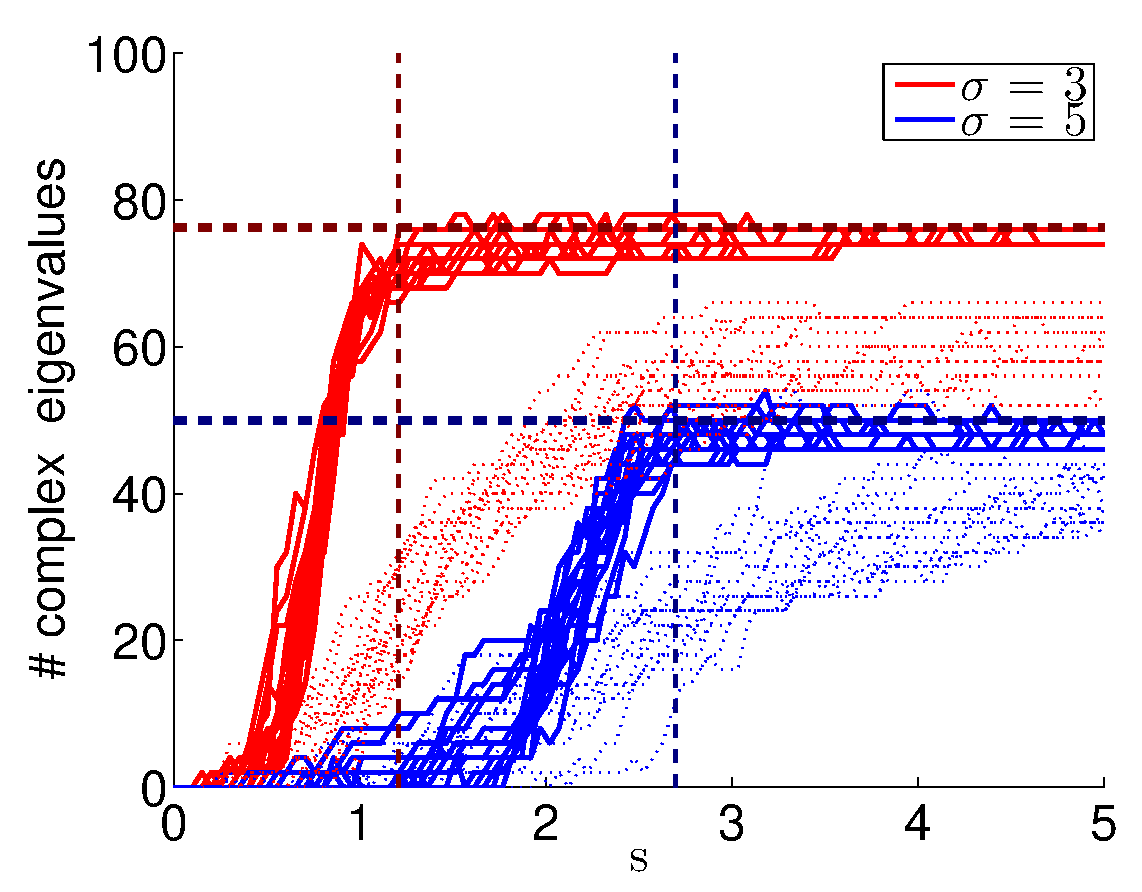
\includegraphics[height=4cm]{numComplex_100_alpha_sigma}

\emp

\esl


\bslC

\Tl{\large Summary}

\Cn{
\begin{table*}

\begin{tabular}{|c|c|c|l|}
\hline 
Type of disorder & Parameters &  $s_c$ & Remarks  \\ 
\hline
Resistor-network disorder & $\alpha{<}\frac{1}{2}, \ \sigma{=}0$    &  $s_c = \infty$ &  non-percolating    \\
Resistor-network disorder & $\frac{1}{2}{<}\alpha{<}1, \ \sigma{=}0$   &  $s_c \sim (1/N)$ & residual percolation\\
Sparse disorder & $(M/N) \ll 1$ &  $s_c \sim (1/N)$  &  both disorder types   \\
Stochastic field disorder & $\alpha{>}1, \ \sigma{\ne}0$ & $s_c \approx s_{1/2}$ & percolating \\
\hline
\end{tabular}
\end{table*}
}

\begin{itemize}

\item Relaxation properties of a closed circuit, 
whose dynamics is generated by a conservative rate-equation,  
is dramatically different from that of a biased non-hermitian Hamiltonian. 

\item \cgreen{Random resistor network} - Transition to complexity happens  for ${\alpha>1/2}$ \cred{{\bf before} the  percolation transition}.

\item \cgreen{Random walk in random environment} - Transition to complexity happens  for ${\mu>1/2}$  \cred{{\bf before} the  sliding transition}.
\item \cgreen{ Sparse disorder} - $s_c$  diminishes as $1/N$ for {\bf }.

\item Increasing the bias does not lead to full delocalization, instead \cred {\bf ``complexity saturation"} is observed.

\end{itemize}

\esl

\bslC

\Tl{Motivation}

\begin{itemize}

\item \cgreen{\bf Glassines - log wide distribution of rates}
% (Thermal activation, Quantum tunneling, Multiplicative processes )

\begin{enumerate}
\tiny{
\item A. Amir, Y. Oreg, and Y. Imry, Proceedings of the National Academy of Sciences 109, 1850 (2012)
\item A. Vaknin, Z. Ovadyahu, and M. Pollak, Phys. Rev. Lett. 84, 3402 (2000).
\item A. Amir, Y. Oreg, and Y. Imry, Phys. Rev. Lett. 103, 126403 (2009).
}
\end{enumerate}


\item
\cgreen{\bf Non Hermitian QM}


{\bf Vortex depinning in type II superconductors (\cred{$s=$ applied transverse magnetic field})}


\begin{enumerate}
\tiny{
\item N. Hatano and D. R. Nelson, Phys. Rev. Lett. 77, 570 (1996), Phys. Rev. B 56, 8651 (1997).
}
 \end{enumerate}


{\bf Follow ups}

\begin{enumerate}
\tiny{
\item P. W. Brouwer, P. G. Silvestrov, and C. W. J. Beenakker, Phys.
Rev. B 56, R4333 (1997).
\item I. Y. Goldsheid and B. A. Khoruzhenko, Phys. Rev. Lett. 80,
2897 (1998).
\item J. Feinberg and A. Zee, Phys. Rev. E 59, 6433 (1999).
\item  L. G. Molinari, Linear Algebra and its Applications 429, 2221
(2008).
}
\end{enumerate}



\item
\cgreen{\bf Biophysics}

{\bf Pulling pinned polymers, DNA denaturation (\cred{$s=$ pulling force}) }

\begin{enumerate}
\tiny{
\item  D. K. Lubensky and D. R. Nelson, Phys. Rev. Lett. 85, 1572
(2000), Phys. Rev. E 65, 031917
(2002).
}
\end{enumerate}

{ \bf Population biology (\cred{$s=$ convective flow of bacteria relative to the nutrients})}


\begin{enumerate}
\tiny{
\item D. R. Nelson and N. M. Shnerb, Phys. Rev. E 58, 1383 (1998).
\item K. A. Dahmen, D. R. Nelson, and N. M. Shnerb, in Statistical
mechanics of biocomplexity (Springer, 1999) pp. 124�151.
}
\end{enumerate}


{\bf Molecular motors (\cred{$s=$ affinity of chemical cycle})}

\begin{enumerate}
\tiny{
\item  M. E. Fisher,  A. B. Kolomeisky, The force exerted by a molecular motor. PNAS 96, 6597�6602 (1999).
\item Rief, M. et al. Myosin-v stepping kinetics: a molecular model for processivity. PNAS 97, 9482�9486 (2000).
\item Y. Kafri, D. K. Lubensky, and D. R. Nelson, Biophysical Journal 86, 3373 (2004), Phys. Rev. E 71, 041906 (2005).
}
\end{enumerate}
\end{itemize}
\esl

\end{document}


